The scenario risk calculator computes loss statistics for all \glspl{asset} in
a given \gls{exposuremodel} for a single specified \gls{rupture}.
Loss statistics include the mean and standard deviation of ground-up losses
and insured losses for each loss type considered in the analysis. Loss
statistics can currently be computed for five different loss types using this
calculator: structural losses, nonstructural losses, contents losses, downtime
losses, and occupant fatalities. This calculator requires the definition of a
finite \gls{rupturemodel}, an \gls{exposuremodel} and a
\gls{vulnerabilitymodel} for each loss type considered; the main results are
the loss statistics per \gls{asset} and mean loss maps.

The \gls{rupture} characteristics---i.e. the magnitude, hypocenter and fault
geometry---are modelled as deterministic in the scenario calculators. Multiple
realizations of different possible \glspl{acr:gmf} due to the single
\gls{rupture} are generated, taking into consideration both the inter-event
variability of ground motions, and the intra-event residuals obtained from a
spatial correlation model for ground motion residuals. The use of logic trees
allows for the consideration of uncertainty in the choice of a ground motion
model for the given tectonic region.

As an alternative to computing the \glspl{acr:gmf} with OpenQuake, users can
also provide their own sets of \glspl{acr:gmf} as input to the scenario risk
calculator.

For each \gls{acr:gmf} realization, a loss ratio is sampled for every asset in
the \gls{exposuremodel} using the provided probabilistic
\gls{vulnerabilitymodel} taking into consideration the correlation model for
vulnerability of different \glspl{asset} of a given taxonomy. Finally loss
statistics, i.e., the mean loss and standard deviation of loss for both
ground-up losses and insured losses across all realizations, are calculated
for each \gls{asset}. Mean loss maps are also generated by this calculator,
describing the mean ground-up losses and mean insured losses caused by the
scenario event for the different assets in the \gls{exposuremodel}.

The required input files required for running a scenario risk calculation and
the resulting output files are depicted in Figure~\ref{fig:io-structure-scenario-risk}.

\begin{figure}[ht]
\centering
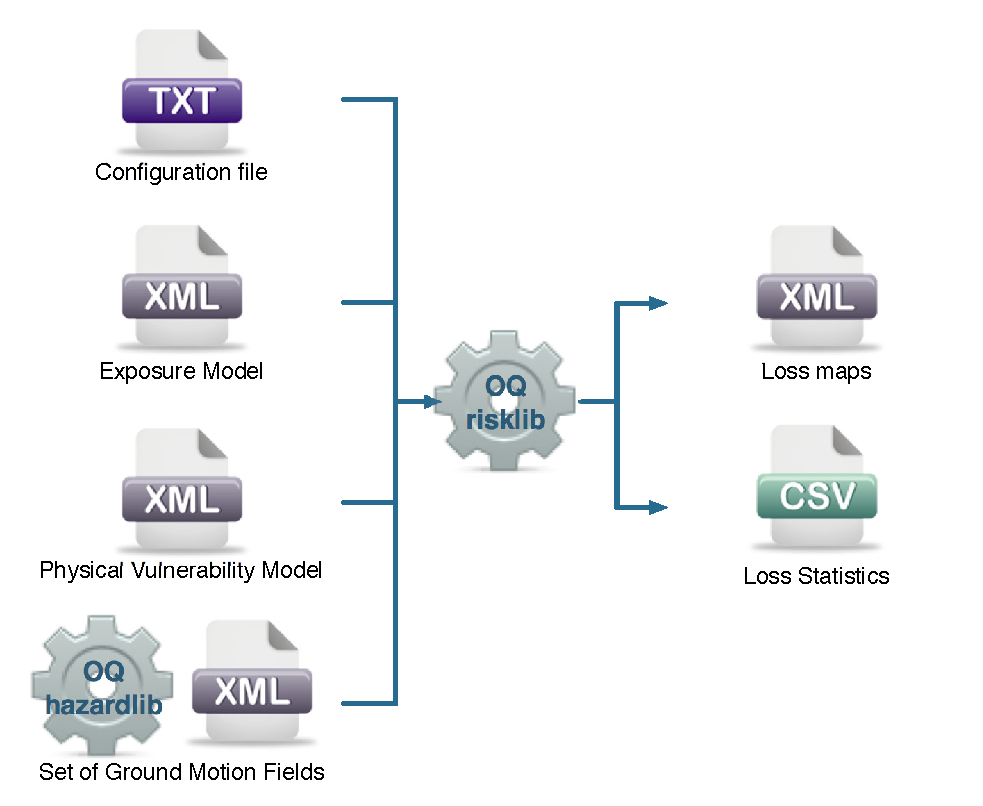
\includegraphics[width=9cm,height=7cm]{figures/risk/io-structure-scenario-risk.pdf}
\caption{Scenario Risk Calculator input/output structure.}
\label{fig:io-structure-scenario-risk}
\end{figure}